\documentclass[twoside]{article}

% We add packages, macros here:
%!TEX root =  lec-template.tex
\usepackage{lmodern}
\usepackage[english]{babel}
\usepackage{latexsym}
\usepackage{amsmath}
\usepackage{mathrsfs}
\usepackage{amssymb}
\usepackage{mathtools}
\usepackage[inline,shortlabels]{enumitem} % we prefer enumitem because of its margin adjustment caps
\usepackage{bm}
\usepackage{datetime}
\usepackage[table,xcdraw]{xcolor}
\usepackage{accents}
\usepackage{tikz}
\usepackage{listings}
\usepackage{mdframed}
\usepackage{pgfplots}
\usepackage{pgfplotstable}
\usepackage[boxed]{algorithm}
\usepackage{algpseudocode}
\usepackage{dsfont}
\usepackage{color}
\usepackage{colortbl}
\usepackage{pifont}
\usepackage[bf,font=small,singlelinecheck=off]{caption}
\usepackage{microtype} % improved spacing between words for easier reading
\usepackage{float}
\usepackage{xfrac} % sfrac
\usepackage{xspace}

\linespread{1.1}


\usepackage[textsize=tiny]{todonotes}
\makeatletter
\renewcommand{\todo}[2][]{\@todo[#1]{#2}}
\makeatother

\setlength{\marginparwidth}{10ex}
\newcommand{\todoc}[2][]{\todo[size=\scriptsize,color=blue!20!white,#1]{Csaba: #2}}
\newcommand{\todoj}[2][]{\todo[size=\scriptsize,color=red!20!white,#1]{Jincheng: #2}}

\usepackage{hyperref}
\hypersetup{
    unicode=false,          % non-Latin characters in Acrobat�s bookmarks
    pdftoolbar=true,        % show Acrobat�s toolbar?
    pdfmenubar=true,        % show Acrobat�s menu?
    pdffitwindow=false,     % window fit to page when opened
    pdfstartview={FitH},    % fits the width of the page to the window
    pdftitle={},    % title
    pdfauthor={},     % author
    pdfsubject={Theory, Machine Learning, Lectures},   % subject of the document
    pdfcreator={},   % creator of the document
    pdfproducer={}, % producer of the document
    pdfkeywords={theory} {machine learning} {lecture notes} {CMPUT 654} {Fall 2023}, % list of keywords
    pdfnewwindow=true,      % links in new window
    colorlinks=true,       % false: boxed links; true: colored links
    linkcolor=blue,          % color of internal links (change box color with linkbordercolor)
    citecolor=blue,        % color of links to bibliography
    filecolor=magenta,      % color of file links
    urlcolor=cyan           % color of external links
}
\usepackage{amsthm}
\usepackage{times}
\usepackage{natbib}
\usepackage{nicefrac}
\usepackage{wrapfig}
\usepackage[capitalize]{cleveref}
\usepackage[nottoc,numbib]{tocbibind}

%\usepackage[bmargin=0.75in]{geometry}
\usepackage[margin=1.1in]{geometry}
\usepackage[normalem]{ulem}


%%%%%%%%%%%%%%%%%%%%%%%%%%%%%%%%
% HYPHENATION
%%%%%%%%%%%%%%%%%%%%%%%%%%%%%%%%

\pretolerance=5000
\tolerance=9000
\emergencystretch=0pt
\righthyphenmin=4
\lefthyphenmin=4


\bibliographystyle{plainnat}

\newcommand{\E}{\mathbb{E}}
\newcommand{\EE}[1]{\E[#1]}
\newcommand{\PP}{\mathbb{P}}
\newcommand{\Prob}[1]{\mathbb{P}(#1)}
\newcommand{\one}[1]{\mathbb{I}\{#1\}}
\newcommand{\Supp}{\operatorname{supp}}
\newcommand{\ip}[1]{\langle #1 \rangle}
\newcommand{\bip}[1]{\left\langle #1 \right\rangle}
\newcommand{\norm}[1]{\|#1\|}
\newcommand{\R}{\mathbb{R}}
\newcommand{\N}{\mathbb{N}}
\newcommand{\cA}{\mathcal{A}}
\newcommand{\cB}{\mathcal{B}}
\newcommand{\cC}{\mathcal{C}}
\newcommand{\cD}{\mathcal{D}}
\newcommand{\cE}{\mathcal{E}}
\newcommand{\cF}{\mathcal{F}}
\newcommand{\cG}{\mathcal{G}}
\newcommand{\cH}{\mathcal{H}}
\newcommand{\cK}{\mathcal{K}}
\newcommand{\cL}{\mathcal{L}}
\newcommand{\cN}{\mathcal{N}}
\newcommand{\cP}{\mathcal{P}}
\newcommand{\cQ}{\mathcal{Q}}
\newcommand{\cR}{\mathcal{R}}
\newcommand{\cS}{\mathcal{S}}
\newcommand{\sA}{\mathscr A}

\newcommand{\cM}{\mathcal{M}}
\newcommand{\cX}{\mathcal{X}}
\newcommand{\cY}{\mathcal{Y}}
\newcommand{\NN}{\mathbb{N}}
\newcommand{\RR}{\mathbb{R}}
\newcommand{\VV}[1]{\mathbb{V}[#1]}

\newcommand{\epsapp}{\epsilon}
\newcommand{\epssub}{\delta}

\DeclareMathOperator{\Range}{range}
\newcommand{\rows}{\operatorname{rows}}

\renewcommand{\epsilon}{\varepsilon}
\newcommand{\ceil}[1]{\left\lceil {#1} \right\rceil}
\newcommand{\floor}[1]{\left\lfloor {#1} \right\rfloor}
\newcommand{\ones}{\mathbf{1}}
\newcommand{\zeros}{\mathbf{0}}
\DeclareMathOperator*{\argmin}{arg\ min}
\DeclareMathOperator*{\argmax}{arg\ max}


\def\rvzero{{\mathbf{0}}}
\def\rvone{{\mathbf{1}}}

\def\identiymatrix{\mathbf{Id}}

\newcommand{\softmax}{\mathrm{softmax}}
\newcommand{\KL}{D_{\mathrm{KL}}}

% Graph
\def\gA{{\mathcal{A}}}
\def\gB{{\mathcal{B}}}
\def\gC{{\mathcal{C}}}
\def\gD{{\mathcal{D}}}
\def\gE{{\mathcal{E}}}
\def\gF{{\mathcal{F}}}
\def\gG{{\mathcal{G}}}
\def\gH{{\mathcal{H}}}
\def\gI{{\mathcal{I}}}
\def\gJ{{\mathcal{J}}}
\def\gK{{\mathcal{K}}}
\def\gL{{\mathcal{L}}}
\def\gM{{\mathcal{M}}}
\def\gN{{\mathcal{N}}}
\def\gO{{\mathcal{O}}}
\def\gP{{\mathcal{P}}}
\def\gQ{{\mathcal{Q}}}
\def\gR{{\mathcal{R}}}
\def\gS{{\mathcal{S}}}
\def\gT{{\mathcal{T}}}
\def\gU{{\mathcal{U}}}
\def\gV{{\mathcal{V}}}
\def\gW{{\mathcal{W}}}
\def\gX{{\mathcal{X}}}
\def\gY{{\mathcal{Y}}}
\def\gZ{{\mathcal{Z}}}

% Sets
\def\sA{{\mathbb{A}}}
\def\sB{{\mathbb{B}}}
\def\sC{{\mathbb{C}}}
\def\sD{{\mathbb{D}}}
% Don't use a set called E, because this would be the same as our symbol
% for expectation.
\def\sE{{\mathbb{E}}}
\def\sF{{\mathbb{F}}}
\def\sG{{\mathbb{G}}}
\def\sH{{\mathbb{H}}}
\def\sI{{\mathbb{I}}}
\def\sJ{{\mathbb{J}}}
\def\sK{{\mathbb{K}}}
\def\sL{{\mathbb{L}}}
\def\sM{{\mathbb{M}}}
\def\sN{{\mathbb{N}}}
\def\sO{{\mathbb{O}}}
\def\sP{{\mathbb{P}}}
\def\sQ{{\mathbb{Q}}}
\def\sR{{\mathbb{R}}}
\def\sS{{\mathbb{S}}}
\def\sT{{\mathbb{T}}}
\def\sU{{\mathbb{U}}}
\def\sV{{\mathbb{V}}}
\def\sW{{\mathbb{W}}}
\def\sX{{\mathbb{X}}}
\def\sY{{\mathbb{Y}}}
\def\sZ{{\mathbb{Z}}}

\newcommand{\dimE}{\mathrm{dim}_{\mathcal{E}}}
\DeclareMathOperator{\diam}{diam}


%%
%% ADD PACKAGES here:
%%
%
%\usepackage{amsmath,amsfonts,graphicx}
%
%
% The following commands set up the lecnum (lecture number)
% counter and make various numbering schemes work relative
% to the lecture number.
%

\newcounter{lecnum}
\renewcommand{\thepage}{\thelecnum-\arabic{page}}
\renewcommand{\thesection}{\thelecnum.\arabic{section}}
\renewcommand{\theequation}{\thelecnum.\arabic{equation}}
\renewcommand{\thefigure}{\thelecnum.\arabic{figure}}
\renewcommand{\thetable}{\thelecnum.\arabic{table}}


%
% The following macro is used to generate the header.
%
\newcommand{\lecture}[4]{
   \pagestyle{myheadings}
   \thispagestyle{plain}
   \newpage
   \setcounter{lecnum}{#1}
   \setcounter{page}{1}
   \noindent
   \begin{center}
   \framebox{
      \vbox{\vspace{2mm}
    \hbox to 6.28in { {\bf CMPUT 654 Fa 23: Theoretical Foundations of Machine Learning \hfill Fall 2023} }
       \vspace{4mm}
       \hbox to 6.28in { {\Large \hfill Lecture #1: #2  \hfill} }
       \vspace{2mm}
       \hbox to 6.28in { {\it Lecturer: #3 \hfill Scribes: #4} }
      \vspace{2mm}}
   }
   \end{center}
   \markboth{Lecture #1: #2}{Lecture #1: #2}

   \noindent {\bf Note}: {\it 
   \LaTeX\  template courtesy of UC Berkeley EECS dept. (\href{https://inst.eecs.berkeley.edu/~cs294-8/sp03/Materials/}{link} to directory)
   }

   \noindent {\bf Disclaimer}: {\it These notes have \underline{\textbf{not}} been subjected to the
   usual scrutiny reserved for formal publications. They may be
   distributed outside this class only with the permission of the
   Instructor.} \vspace*{4mm}
}
%
% Convention for citations is authors' initials followed by the year.
% For example, to cite a paper by Leighton and Maggs you would type
% \cite{LM89}, and to cite a paper by Strassen you would type \cite{S69}.
%%%%%%%%% (To avoid bibliography problems, for now we redefine the \cite command.)
%%%%%%%%% Also commands that create a suitable format for the reference list.
%%%%%%%%\renewcommand{\cite}[1]{[#1]}
%%%%%%%%\def\beginrefs{\begin{list}%
%%%%%%%%        {[\arabic{equation}]}{\usecounter{equation}
%%%%%%%%         \setlength{\leftmargin}{2.0truecm}\setlength{\labelsep}{0.4truecm}%
%%%%%%%%         \setlength{\labelwidth}{1.6truecm}}}
%%%%%%%%\def\endrefs{\end{list}}
%%%%%%%%\def\bibentry#1{\item[\hbox{[#1]}]}

%Use this command for a figure; it puts a figure in wherever you want it.
%usage: \fig{NUMBER}{SPACE-IN-INCHES}{CAPTION}
\newcommand{\fig}[3]{
			\vspace{#2}
			\begin{center}
			Figure \thelecnum.#1:~#3
			\end{center}
	}
% Use these for theorems, lemmas, proofs, etc.

%!TEX root =  lec-template.tex
%%%%%%%%%%%%%%%%%%%%%%%%%%%%%%%%
% THEOREMS
%%%%%%%%%%%%%%%%%%%%%%%%%%%%%%%%
\theoremstyle{plain}
\newtheorem{theorem}{Theorem}[lecnum]
\newtheorem{claim}[theorem]{Claim}
\newtheorem{proposition}[theorem]{Proposition}
\newtheorem{lemma}[theorem]{Lemma}
\newtheorem{corollary}[theorem]{Corollary}
\newtheorem{example}[theorem]{Example}
\theoremstyle{definition}
\newtheorem{definition}[theorem]{Definition}
\newtheorem{assumption}[theorem]{Assumption}
\newtheorem{remark}[theorem]{Remark}
\newtheorem{exercise}[theorem]{Exercise}
\theoremstyle{remark}


%\newtheorem{theorem}{Theorem}[lecnum]
%\newtheorem{lemma}[theorem]{Lemma}
%\newtheorem{proposition}[theorem]{Proposition}
%\newtheorem{claim}[theorem]{Claim}
%\newtheorem{corollary}[theorem]{Corollary}
%\newtheorem{definition}[theorem]{Definition}
%\newenvironment{proof}{{\bf Proof:}}{\hfill\rule{2mm}{2mm}}

% **** IF YOU WANT TO DEFINE ADDITIONAL MACROS FOR YOURSELF, PUT THEM HERE:

\newcommand{\set}[1]{\left\{#1\right\}}
\newcommand{\I}{\mathbb{I}}


\begin{document}
%FILL IN THE RIGHT INFO.
%\lecture{**LECTURE-NUMBER**}{**DATE**}{**LECTURER**}{**SCRIBE**}
\lecture{7}{September 26}{Csaba Szepesv\'ari}{Kushagra Chandak}
%\footnotetext{These notes are partially based on those of Nigel Mansell.}

% **** YOUR NOTES GO HERE:

% Some general latex examples and examples making use of the
% macros follow.  
%**** IN GENERAL, BE BRIEF. LONG SCRIBE NOTES, NO MATTER HOW WELL WRITTEN,
%**** ARE NEVER READ BY ANYBODY.

\section{Outline}
\begin{itemize}[-]
    \item Recap of lower bracketing cover and using it in Chernoff bounds.
    \item Linear threshold class example.
    \item Bounded variance class.
\end{itemize}

\section{Recap}
In the last lecture, we started talking about infinite function classes and the fact that we just need to account for a finite \emph{cover} of the infinite function class in the union bound to get uniform deviation bounds. The covering happens at some accuracy or \emph{scale} $\varepsilon$, and there is a tradeoff between the approximation error introduced by $\varepsilon$ and the number of elements in the cover.  

We also talked about the \emph{lower bracketing cover} which is useful in obtaining one-sided uniform deviation bounds. Recall the setting for defining a lower bracketing cover:  Let $\cG \subseteq \R^{\cZ}$ and $P \in \cM_1(\cZ)$.
\begin{definition}[Lower bracketing cover]
     Fix $\varepsilon > 0$. Then $g_1, \dots, g_m : \cZ \to \R$ is a lower bracketing cover of $\cG$ with distribution $P$ and scale $\varepsilon$ (shorthand: $\cG @ P @ \varepsilon$) such that for any $g \in \cG$ there exists $j \in [m]$ such that: (1) $g_j \le g$; and (2) $Pg \le Pg_j + \varepsilon$.
\end{definition}
The minimum number of functions in the lower bracketing cover is called the lower bracketing number denoted by $N_{\varepsilon} = N_{\text{LB}}(\varepsilon, \cG, P)$. Note that the cover $g_1,\dots,g_m$ may or may not be in $\cG$. A lower bracketing cover can be used for one-sided uniform deviations, which we used to analyze ERM.  

Further, recall that the empirical distribution is given by $P_n = \frac1n \sum_{i=1}^n \delta_{z_i}$ where $z_1,\dots,z_n \sim P$ iid. Then the ERM is
\[
    \hat{g}_n = \argmin_{g \in \cG} P_n g \,,
\]
which implicitly selects a predictor that underlies the loss. Using Chernoff's inequality, we get the following bound for ERM.
\begin{proposition}
    Let $\cG \subseteq [0,1]^{\cZ}$. For every $\delta \in (0,1)$:
    \begin{enumerate}
        \item w.p. $1-\delta$, $P\hat{g}_n \le \inf_{g \in \cG} Pg + \inf_{\varepsilon > 0} \left( \varepsilon + 2 \sqrt{\frac{\ln (N_{\varepsilon}+1)/\delta}{2n}} \right)$.
        \item for every $\varepsilon > 0$,  w.p. $1-\delta$, $P\hat{g}_n \le \inf_{g \in \cG} \left(Pg + \sqrt{\frac{2Pg \ln (N_{\varepsilon}+1)/\delta}{n}} \right) + \varepsilon + \sqrt{\frac{2P\hat{g}_n \ln (N_{\varepsilon}+1)/\delta}{n}} + \frac{\ln(N_{\varepsilon}+1)/\delta}{3n}$.
    \end{enumerate}
\end{proposition}
\begin{remark}
    \begin{enumerate}
        \item For the second bound above, we did not take $\inf$ over $\varepsilon > 0$ in the RHS, since $P\hat{g}_n$ is random on the RHS. But we can first solve for $\inf$ over $\cG$, solve a quadratic to get a bound for $P\hat{g}_n$, and then take the $\inf$ over $\varepsilon$.
        \item If $g_1, \dots, g_m$ were chosen from the class $\cG$, then the size of the cover might increase slightly and we might lose some constant factors in the bounds.
    \end{enumerate}
\end{remark}

% \textbf{Discussion. } Recall that for the finite class case, an inequality for one side was used for a specific function. And for other side of the inequality, we used a uniform bound. In the above inequalities, we used only one-sided uniform bouonds.

\section{Covering the Linear Threshold Class}
\paragraph{Setting.} 
Let $\cX = [0,1]$ and $\cY \in \set{0,1}$. Let the function class be $\cF = \set{f_w: \cX \to \cY : w \in [0,1] }$ where $f_w(x) = \I( x \ge w)$ is the \emph{linear threshold function} (\cref{fig:thresh-fn}). We consider the zero-one loss where the loss class is defined as $\cG = \set{\ell_{01} \circ f_w : w \in [0,1]}$. The loss function is a map $\ell_{01} \circ f_w: \cX \times \set{0,1} \to \set{0,1}$ defined as $(x,y) \mapsto \I(f(x) \ne y)$. We also write the loss $\ell_{01} \circ f_w$ as $g_w$.

\begin{figure}
    \centering
    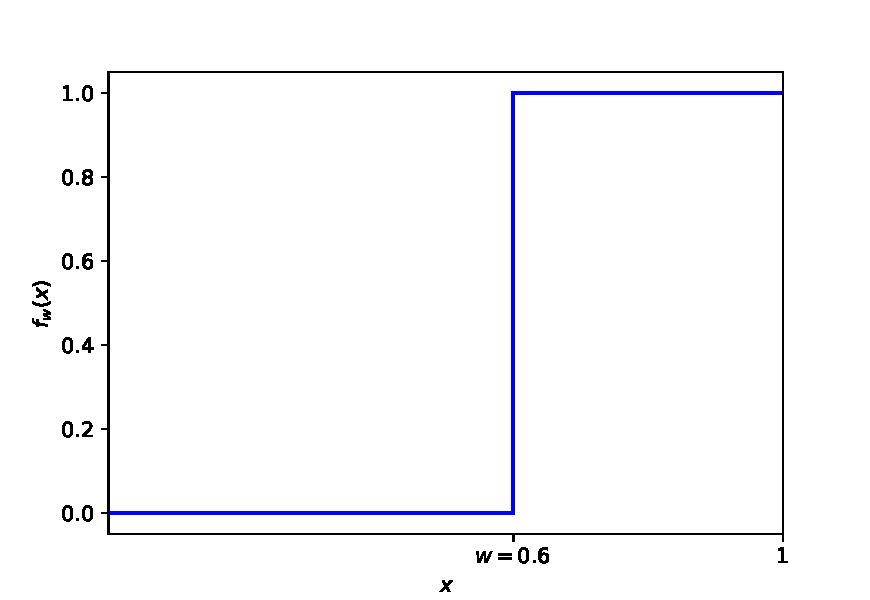
\includegraphics[width=12cm, height=6cm]{figures/threshold_fn.pdf}
     \caption{An example of a linear threshold function $f_w(x) = \I(x \ge w)$ with $w = 0.6$.}
    \label{fig:thresh-fn}
\end{figure}

\paragraph{Lower bracketing cover.}
We first discretize the one-dimensional space of $w$'s at the scale of $\varepsilon$. Let $w_j = \set{\varepsilon, 2\varepsilon, \dots, N_{\varepsilon}\varepsilon}$, where $N_{\varepsilon} = \lceil \frac{1}{\varepsilon} \rceil$.

The elements of the cover are given by $g_j = g_{w_j}\I( x \notin [w_j-\varepsilon, w_j])$. To check the first condition for a lower bracketing cover, notice that for any function $g_{w}$, outside $[w_j-\varepsilon, w_j]$ we have $g_w = g_{w_j}$  as $f_w = f_{w_j}$. Inside $[w_j-\varepsilon, w_j]$, we have $g_i = 0$ by definition. Therefore $g_i \le g_w$. To check the second condition for a lower bracketing cover, we follow the same argument as above and notice that the length of the interval $[w_j-\varepsilon, w_j]$ is $\varepsilon$ and the difference between $g_w$ and $g_j$ is bounded by 1, which gives $Pg_w \le Pg_i + \varepsilon$. We illustrate these conditions in \cref{fig:lb}.

\begin{figure}
    \centering
    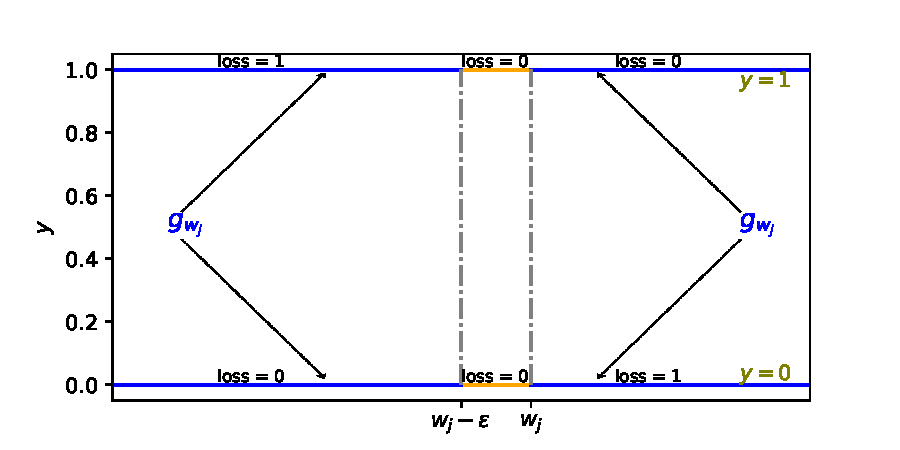
\includegraphics[width=12cm, height=6cm]{figures/loss.pdf}
     \caption{Lower bracketing cover for linear threshold functions. The goal is to cover a function $g_w$ so that $w \in [w_j-\varepsilon, w_j]$. The cover element is $g_j = w_j \I(x \not in [w_j-\varepsilon, w_j])$. The indicated losses are for $g_j$ for the cases $y=0$ and $y=1$. The blue horizontal lines show the function. The blue horizontal lines indicate the intervals on which $g_j = g_{w_j}$ and the orange lines show the interval when $g_j = 0$.}
    \label{fig:lb}
\end{figure}

We can also define two-sided bracketing.
\begin{definition}[Bracketing]
    Fix $\varepsilon > 0$. The functions $g_1^U, \dots, g_m^U$ and $g_1^L, \dots, g_m^L$ from $\cZ \to \R$ is a cover of $\cG @ P @ \varepsilon$ if $\forall g \in \cG$ there exists $j \in [m]$ such that (1) $g_j^L \le g \le g_j^U$; and (2) $Pg_j^U - \varepsilon \le Pg \le Pg_j^L + \varepsilon$ (\textcolor{red}{CHECK!}).
\end{definition}
We remark that we lose some constant factors in the bounds while using bracketing.

\section{Bounded Variance Condition}
Multiplicative Chernoff gave fast convergence rates ($1/n$), however, it was restricted to the case when the predictors/losses are bounded and the loss is small. For some special cases when the variance of the loss is bounded, we can still get fast rates by exploiting the bounded variance property. This is given by Bernstein's inequality. But before delving into Bernstein's, let us define the bounded variance class and discuss some examples of loss classes that have bounded variance.   


Let $\cZ = \cX \times \cY$ for some sets $\cX, \cY$ and $g:\cZ \to \cR$ be a measurable function. Further, let $P \in \cM_1(\cZ)$. The variance of $g$ measured against $P$ is given by $\Var_P(g) = P(g-Pg)^2$.

\begin{definition}[Bounded variance class]
    Fix $c_0, c_1 > 0$. Then the bounded variance class is defined as
    \[
        Var_{\cZ}(c_0, c_1, P) = \set{g: \cZ \to \R : \Var_P(g) \le c_0^2 + c_1Pg } \,.
    \]
\end{definition}

\paragraph{Examples.}
\begin{enumerate}
    \item \textbf{Bounded functions.} If $0 \le g \le 1$, then $g \in \Var_{\cZ}(0, 1, P)$.

    \item \textbf{Convex function class. }
    For some set $\cX$, let $\cF \subset \cM(\cX,\R)$ and assume that $\cF$ is convex (i.e., for any $\alpha\in [0,1]$, $f,g\in \cF$, $\alpha f + (1-\alpha)g \in \cF$ also holds).
    Let $\cZ = \cX \times \R$ and 
    \[
        \cG = \{ \ell_f \,:\, \ell_f: \cZ \to \R, \ell_f(x,y) = (f(x)-y)^2, f\in \cF \}\,.
    \]
    By abusing notation, we also write for this set  $\cG = \ell_{\text{sq}}\circ \cF$.
    Let $P\in \cM_1(\cZ)$ be such that
    for some $M>0$ constant, for any $g\in \cG$, $g(Z)\le M^2$ with probability one, where $Z\sim P$.
    Define $g_* = \argmin_{g\in \cG} P g$ (which is assumed to exist) and 
    \begin{align*}
    \tilde\cG = \{ g - g_* \,:\, g\in \cG \}  \quad (= \cG - \{ g_*\})\,,
    \end{align*}
    so that $\inf_{\tilde{g} \in \tilde{\cG}} P\tilde{g} = 0$. Then, 
    \begin{align*}
    \tilde \cG \subset \Var_{\cZ}(0, 4M^2,P).
    \end{align*}

    \item \textbf{Best predictor not in the function class. }
    Fix $M>0$. Let $\cF \subset \cM(\cX,[0,M])$ be set set of functions bounded in the interval $[0,M]$, $\cZ = \cX \times [0,M]$, $P\in \cM_1(\cZ)$ be a probability distribution over $\cZ$.
    
    Now let $\cG = \ell_{\text{sq}} \circ \cF$ and $f_*(x) = \EE{Y|X=x}$ for $x\in \cX$ be the best predictor which may not be in the $\cF$. Define
    \[
        \tilde \cG = \cG - \{ \ell_{f_*} \}\,.
    \]
    Then,
    \[
        \tilde \cG \subset \Var_{\cZ}(0, 2M^2,P) \,.
    \]  
\end{enumerate}

 
\end{document}
